\documentclass[12pt,a4paper]{article}

% ─── Packages ────────────────────────────────────────────────────────────────
\usepackage[a4paper, top=2cm, bottom=2.2cm, left=2.2cm, right=2.2cm]{geometry}
\usepackage[utf8]{inputenc}
\usepackage[T1]{fontenc}
\usepackage{lmodern}
\usepackage{microtype}
\usepackage{xcolor}
\usepackage{listings}
\usepackage{enumitem}
\usepackage{titlesec}
\usepackage{fancyhdr}
\usepackage{amsmath}
\usepackage{amssymb}
\usepackage{tcolorbox}
\usepackage{parskip}
\usepackage{tikz}
\usepackage{graphicx}
\usepackage{hyperref}
\usetikzlibrary{arrows.meta, positioning, shapes.geometric, backgrounds, fit, decorations.pathreplacing}

\DeclareUnicodeCharacter{2014}{---}
\DeclareUnicodeCharacter{2013}{--}
\DeclareUnicodeCharacter{2192}{$\to$}
\DeclareUnicodeCharacter{2202}{$\partial$}
\DeclareUnicodeCharacter{2500}{-}
\DeclareUnicodeCharacter{2550}{=}
\DeclareUnicodeCharacter{00B7}{$\cdot$}

% ─── Colours ─────────────────────────────────────────────────────────────────
\definecolor{deepblue}{HTML}{1A237E}
\definecolor{teal}{HTML}{00695C}
\definecolor{orange}{HTML}{BF360C}
\definecolor{green}{HTML}{1B5E20}
\definecolor{red}{HTML}{7B0000}
\definecolor{codebg}{HTML}{F0F2F5}
\definecolor{codeframe}{HTML}{B0BEC5}
\definecolor{kwcolor}{HTML}{0D47A1}
\definecolor{strcolor}{HTML}{B71C1C}
\definecolor{cmtcolor}{HTML}{558B2F}
\definecolor{builtincolor}{HTML}{6A1B9A}
\definecolor{numcolor}{HTML}{004D40}
\definecolor{defselfcolor}{HTML}{1565C0}
\definecolor{noteblue}{HTML}{E3F2FD}
\definecolor{noteborderblue}{HTML}{1565C0}
\definecolor{warnbg}{HTML}{FFF9C4}
\definecolor{warnborder}{HTML}{F57F17}
\definecolor{tipbg}{HTML}{E8F5E9}
\definecolor{tipborder}{HTML}{2E7D32}
\definecolor{dangerbg}{HTML}{FCE4EC}
\definecolor{dangerborder}{HTML}{AD1457}
\definecolor{mathbg}{HTML}{EDE7F6}
\definecolor{mathborder}{HTML}{4527A0}
\definecolor{conceptbg}{HTML}{E0F2F1}
\definecolor{conceptborder}{HTML}{00796B}
\definecolor{stickycolor}{HTML}{FFF176}
\definecolor{stickyborder}{HTML}{F9A825}
\definecolor{patternbg}{HTML}{FFF3E0}
\definecolor{patternborder}{HTML}{E65100}

% ─── Python listings style ────────────────────────────────────────────────────
\lstdefinestyle{py}{
  language=Python,
  backgroundcolor=\color{codebg},
  frame=single, framesep=6pt, rulecolor=\color{codeframe},
  basicstyle=\ttfamily\footnotesize,
  keywordstyle=\color{kwcolor}\bfseries,
  stringstyle=\color{strcolor},
  commentstyle=\color{cmtcolor}\itshape,
  numberstyle=\tiny\color{gray},
  numbers=left, numbersep=8pt, stepnumber=1,
  tabsize=4, showspaces=false, showstringspaces=false,
  breaklines=true, captionpos=b,
  morekeywords={self, cls, None, True, False, lambda, yield, assert},
  emph={print,range,len,type,set,list,sum,zip,reversed,isinstance,
        random,math,Value,Neuron,Layer,MLP,Module},
  emphstyle=\color{builtincolor}\bfseries,
  xleftmargin=10pt, xrightmargin=4pt,
  aboveskip=6pt, belowskip=6pt,
}
\lstset{style=py}

\newcommand{\code}[1]{\texttt{\small\color{deepblue}#1}}
\newcommand{\py}[1]{\texttt{\small\color{kwcolor}#1}}

% ─── tcolorbox environments ──────────────────────────────────────────────────
\tcbset{base/.style={
  fonttitle=\bfseries\small,
  left=6pt, right=6pt, top=5pt, bottom=5pt, boxrule=0.6pt,
}}

\newtcolorbox{notebox}[1][]{base,colback=noteblue,colframe=noteborderblue,
  title={Note},#1}
\newtcolorbox{warnbox}[1][]{base,colback=warnbg,colframe=warnborder,
  title={Warning},#1}
\newtcolorbox{tipbox}[1][]{base,colback=tipbg,colframe=tipborder,
  title={Tip},#1}
\newtcolorbox{dangerbox}[1][]{base,colback=dangerbg,colframe=dangerborder,
  title={Common Bug},#1}
\newtcolorbox{mathbox}[2][]{base,colback=mathbg,colframe=mathborder,
  title={Math: #2},#1}
\newtcolorbox{conceptbox}[2][]{base,colback=conceptbg,colframe=conceptborder,
  title={#2},#1}
\newtcolorbox{stickybox}[1][]{base,colback=stickycolor,colframe=stickyborder,
  title={Sticky Point},#1}
\newtcolorbox{intuitionbox}[1][]{base,colback=mathbg!50!white,colframe=mathborder!60!white,
  title={Intuition},#1}
\newtcolorbox{codeexplainbox}[2][]{base,colback=codebg,colframe=deepblue,
  title={Code Walk-Through: #2},#1}
\newtcolorbox{patternbox}[2][]{base,colback=patternbg,colframe=patternborder,
  title={Pattern: #2},#1}
\newtcolorbox{thinkbox}[1][]{base,colback=tipbg!70!white,colframe=tipborder,
  title={Read This Like Code},#1}

% ─── Section formatting ───────────────────────────────────────────────────────
\titleformat{\section}{\color{deepblue}\Large\bfseries}{\thesection.}{0.5em}{}
  [\color{deepblue}\titlerule]
\titleformat{\subsection}{\color{teal}\large\bfseries}{\thesubsection}{0.5em}{}
\titleformat{\subsubsection}{\color{orange}\normalsize\bfseries}{\thesubsubsection}{0.5em}{}
\titlespacing*{\section}{0pt}{18pt}{8pt}
\titlespacing*{\subsection}{0pt}{12pt}{4pt}
\titlespacing*{\subsubsection}{0pt}{8pt}{4pt}

% ─── Header / Footer ─────────────────────────────────────────────────────────
\pagestyle{fancy}
\fancyhf{}
\fancyhead[L]{\small\color{deepblue}\bfseries Micrograd — Neural Network Training From Scratch}
\fancyhead[R]{\small\color{gray}Vatsav Reddy | Prof.\ Praveen Parchuri}
\fancyfoot[C]{\small\color{gray}\thepage}
\renewcommand{\headrulewidth}{0.5pt}
\renewcommand{\footrulewidth}{0.3pt}
\setlength{\headheight}{14.5pt}

% ─── Hyperref ────────────────────────────────────────────────────────────────
\hypersetup{colorlinks=true,linkcolor=deepblue,urlcolor=teal,
  pdftitle={Micrograd Lecture Notes}}

% ─── List settings ───────────────────────────────────────────────────────────
\setlist[itemize]{leftmargin=1.5em,topsep=2pt,itemsep=1pt,parsep=0pt}
\setlist[enumerate]{leftmargin=1.5em,topsep=2pt,itemsep=1pt,parsep=0pt}

% ─── TikZ helpers ─────────────────────────────────────────────────────────────
\tikzstyle{valnode}=[rectangle,draw=deepblue,fill=noteblue,
  rounded corners=4pt,minimum height=1.4cm,minimum width=2.2cm,
  font=\small\bfseries,align=center]
\tikzstyle{opnode}=[circle,draw=orange,fill=warnbg,
  minimum size=0.7cm,font=\small\bfseries]
\tikzstyle{arr}=[-{Stealth},thick,color=deepblue]

% ═════════════════════════════════════════════════════════════════════════════
\begin{document}
% ═════════════════════════════════════════════════════════════════════════════

% ─── Title page ──────────────────────────────────────────────────────────────
\begin{titlepage}
\centering
\vspace*{1.5cm}
{\Huge\bfseries\color{deepblue} Micrograd: Neural Network Training\\[6pt]
From Scratch\par}
\vspace{0.4cm}
{\large\color{gray} Autograd Engine $\cdot$ Backpropagation $\cdot$ MLP Training\par}
\vspace{1.2cm}
\begin{tcolorbox}[colback=deepblue!8,colframe=deepblue,width=0.85\textwidth]
\centering
\textit{``Neural networks are just mathematical expressions.\\
Backpropagation is just the chain rule, applied recursively.\\
Everything else is efficiency.''}
\end{tcolorbox}
\vspace{1.2cm}
{\large\bfseries Author: Vatsav Reddy\par}
{\normalsize Under the guidance of \textbf{Prof.\ Praveen Parchuri}\par}
\vspace{1cm}
{\normalsize\color{gray} Lecture Reference: Andrej Karpathy — ``Building Micrograd''\par}
\vspace{0.8cm}
\begin{tcolorbox}[colback=stickycolor,colframe=stickyborder,width=0.85\textwidth]
\textbf{After reading these notes carefully, you will be able to:}
\begin{itemize}
  \item Read the full micrograd source and understand every line without hesitation
  \item Trace a forward pass and manually reconstruct what every intermediate \code{Value} holds
  \item Trace a backward pass and compute every \code{.grad} by hand
  \item Identify the exact closure that runs at each node and what it deposits
  \item Write your own custom differentiable operations with correct backward passes
  \item Spot the zero-grad bug, the overwrite bug, and the sign bug immediately
  \item Understand why PyTorch's API looks the way it does
\end{itemize}
\end{tcolorbox}
\vfill
{\small\color{gray} Read linearly the first time. Every code block is annotated to build mental models, not just recall.\par}
\end{titlepage}

\tableofcontents
\newpage

% ═════════════════════════════════════════════════════════════════════════════
\section{What Problem Are We Actually Solving?}
% ═════════════════════════════════════════════════════════════════════════════

A neural network is a function. It takes numbers in and produces numbers out. You want it to produce \emph{specific} numbers — the right answers. To get it there, you adjust its internal knobs (the weights) by tiny amounts, over and over. The question is: which direction should each knob turn, and by how much?

That question is exactly what a derivative answers. For a weight $w$ and a loss $L$, $\frac{\partial L}{\partial w}$ tells you exactly how much the loss changes when $w$ changes by a tiny amount. If you know this for every single weight in the network, you know how to adjust all of them in parallel to make the loss go down.

The problem is that a real network might have billions of weights, and the expression connecting them to the loss is enormous. You cannot write out the derivative by hand. You need an algorithm that can compute all these derivatives automatically, for any expression, no matter how complex.

That algorithm is \textbf{backpropagation}. The software machinery that implements it is an \textbf{autograd engine}. Micrograd is a minimal, readable implementation of exactly this — 100 lines of Python.

\begin{stickybox}
Everything in micrograd exists to answer one question: given an output $L$ and any weight $w$ buried deep in the expression that produced $L$, what is $\frac{\partial L}{\partial w}$?
\end{stickybox}

\subsection{The Stack}

\begin{center}
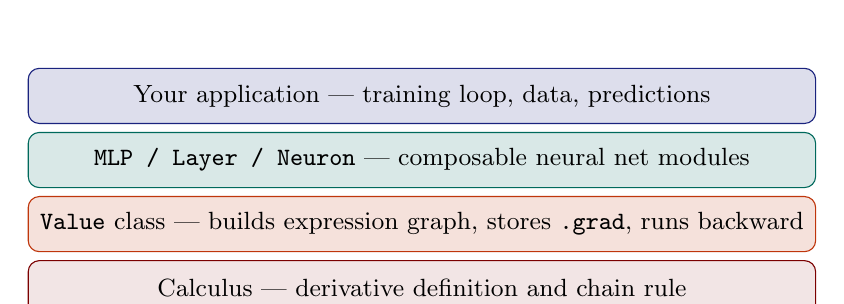
\begin{tikzpicture}[every node/.style={font=\small}]
  \node[fill=deepblue!15,draw=deepblue,rounded corners,minimum width=10cm,
        minimum height=0.7cm,align=center] (l4) {Your application — training loop, data, predictions};
  \node[fill=teal!15,draw=teal,rounded corners,minimum width=10cm,
        minimum height=0.7cm,align=center,below=0.1cm of l4] (l3) {\texttt{MLP / Layer / Neuron} — composable neural net modules};
  \node[fill=orange!15,draw=orange,rounded corners,minimum width=10cm,
        minimum height=0.7cm,align=center,below=0.1cm of l3] (l2) {\texttt{Value} class — builds expression graph, stores \texttt{.grad}, runs backward};
  \node[fill=red!10,draw=red,rounded corners,minimum width=10cm,
        minimum height=0.7cm,align=center,below=0.1cm of l2] (l1) {Calculus — derivative definition and chain rule};
\end{tikzpicture}
\end{center}

Each layer uses the one below it but knows nothing about the ones above. The \code{Value} class does not know what a neuron is. A neuron does not know what a training loop is. This separation is what makes the design clean and reusable.

% ═════════════════════════════════════════════════════════════════════════════
\section{Derivatives — What the Numbers Actually Mean}
% ═════════════════════════════════════════════════════════════════════════════

\subsection{The Definition, Read Carefully}

\begin{mathbox}{Derivative as limit}
\[
\frac{df}{dx}\bigg|_{x=a} = \lim_{h \to 0} \frac{f(a+h) - f(a)}{h}
\]
\end{mathbox}

This formula is not just notation — read it as an instruction. Start at point $a$. Take a tiny step $h$ in the positive $x$ direction. Measure how much $f$ changed. Divide by $h$ to normalize. As $h$ shrinks toward zero, this ratio converges to the derivative.

The derivative is not a property of $f$ globally — it is a number at a specific point. It changes from point to point. At $x=3$, the derivative of $f(x) = 3x^2 - 4x + 5$ is 14. At $x=-3$, it is $-22$. These are completely different numbers describing completely different local behavior.

\begin{intuitionbox}
The derivative tells you three things simultaneously: \textbf{sign} (does $f$ go up or down when you nudge $x$ up?), \textbf{magnitude} (how fast?), and \textbf{locality} (only valid near this specific $x$, not globally). All three matter in training.
\end{intuitionbox}

\subsection{Numerical Estimation — The Sanity Check}

Before any autograd machinery, you can estimate derivatives by literally doing what the definition says: pick a small $h$, evaluate $f$ twice, divide.

\begin{lstlisting}
def f(x):
    return 3*x**2 - 4*x + 5

x = 3.0
h = 0.0001

# Rise over run - the definition, made concrete
slope = (f(x + h) - f(x)) / h
print(slope)   # 14.0002...  (analytically: 6x - 4 = 14 at x=3)
\end{lstlisting}

\begin{codeexplainbox}{Why this is useful but not scalable}
This works for one variable at a time. For a neural net with $N$ parameters, you'd need $N$ forward passes just to estimate the gradient once — astronomically slow. Backpropagation computes all $N$ gradients in roughly the cost of \emph{two} forward passes. That is why we need autograd.

Use numerical estimation to \emph{verify} that your autograd gives correct answers. This is called a gradient check.
\end{codeexplainbox}

\subsection{Partial Derivatives — Multiple Inputs}

When a function has multiple inputs, $\frac{\partial d}{\partial a}$ asks: if only $a$ changes and everything else is fixed, how does $d$ respond?

\begin{lstlisting}
# d = a*b + c
a, b, c = 2.0, -3.0, 10.0
d = a*b + c          # forward: d = 4.0

h = 0.0001

# Partial w.r.t. a: hold b and c fixed, nudge only a
d2 = (a+h)*b + c
print((d2 - d) / h)  # -3.0  - equals b (analytically: dd/da = b)

# Partial w.r.t. b: hold a and c fixed
d2 = a*(b+h) + c
print((d2 - d) / h)  # 2.0   - equals a (analytically: dd/db = a)

# Partial w.r.t. c: trivially 1.0 because d(a*b + c)/dc = 1
d2 = a*b + (c+h)
print((d2 - d) / h)  # 1.0
\end{lstlisting}

\begin{patternbox}{Analytic partial derivatives for common ops}
These are the local gradients you will encounter over and over:
\begin{itemize}
  \item \textbf{Addition} $d = a + b$: $\frac{\partial d}{\partial a} = 1$, $\frac{\partial d}{\partial b} = 1$
  \item \textbf{Multiplication} $d = a \cdot b$: $\frac{\partial d}{\partial a} = b$, $\frac{\partial d}{\partial b} = a$
  \item \textbf{Power} $d = a^n$: $\frac{\partial d}{\partial a} = n \cdot a^{n-1}$
  \item \textbf{ReLU} $d = \max(0, a)$: $\frac{\partial d}{\partial a} = 1$ if $a > 0$, else $0$
\end{itemize}
These are \emph{local} derivatives — they describe only what a single node contributes. To get the full gradient flowing back to a leaf, you chain them with the chain rule.
\end{patternbox}

% ═════════════════════════════════════════════════════════════════════════════
\section{The Chain Rule — The Only Idea Backpropagation Uses}
% ═════════════════════════════════════════════════════════════════════════════

\begin{mathbox}{Chain Rule}
If $z$ depends on $y$ and $y$ depends on $x$:
\[
\frac{dz}{dx} = \frac{dz}{dy} \cdot \frac{dy}{dx}
\]
\end{mathbox}

This extends to any chain of dependencies. If $L$ depends on $d$ which depends on $c$, then $\frac{\partial L}{\partial c} = \frac{\partial L}{\partial d} \cdot \frac{\partial d}{\partial c}$.

The multiplication is the key insight. You do not need to know the full path from $c$ to $L$ at once. You only need two pieces: how $d$ influences $L$ (which arrives as a gradient from upstream), and how $c$ influences $d$ (the local derivative, which the node can compute on its own).

\begin{stickybox}
Every single node in the computation graph independently knows its own local derivative. It does not need to know anything about the rest of the graph. Backpropagation is just every node doing its local job and passing the result upstream. The chain rule says that multiplying these local contributions together gives the correct global gradient.
\end{stickybox}

\subsection{Manual Backpropagation Through a Graph}

Consider $L = d \cdot f$ where $d = c + e$ and $e = a \cdot b$.

\vspace{0.3cm}
\begin{center}
\resizebox{\textwidth}{!}{%
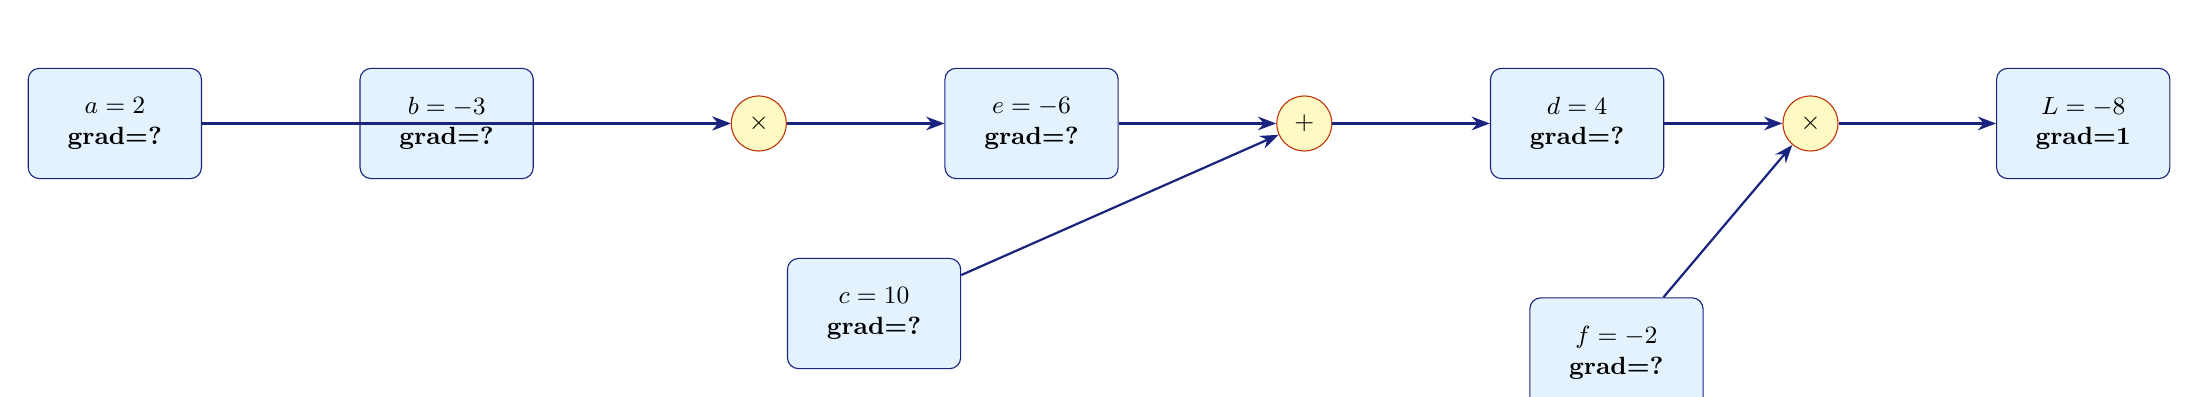
\begin{tikzpicture}[node distance=1.6cm and 2cm]
  \node[valnode] (a) {$a=2$\\grad=?};
  \node[valnode,right=of a] (b) {$b=-3$\\grad=?};
  \node[opnode,right=2.5cm of b] (mul1) {$\times$};
  \node[valnode,right=of mul1] (e) {$e=-6$\\grad=?};
  \node[valnode,below=1cm of e,xshift=-2cm] (c) {$c=10$\\grad=?};
  \node[opnode,right=of e] (plus) {$+$};
  \node[valnode,right=of plus] (d) {$d=4$\\grad=?};
  \node[valnode,below=1.5cm of d,xshift=0.5cm] (f) {$f=-2$\\grad=?};
  \node[opnode,right=1.5cm of d] (mul2) {$\times$};
  \node[valnode,right=of mul2] (L) {$L=-8$\\grad=1};
  \draw[arr] (a) -- (mul1);
  \draw[arr] (b) -- (mul1);
  \draw[arr] (mul1) -- (e);
  \draw[arr] (e) -- (plus);
  \draw[arr] (c) -- (plus);
  \draw[arr] (plus) -- (d);
  \draw[arr] (d) -- (mul2);
  \draw[arr] (f) -- (mul2);
\draw[arr] (mul2) -- (L);
\end{tikzpicture}
}
\end{center}
\vspace{0.3cm}

\textbf{Step 1 — Base case:} $\frac{\partial L}{\partial L} = 1$ always. \code{L.grad = 1}.

\textbf{Step 2 — Multiply node $L = d \cdot f$:} Local derivatives are $\frac{\partial L}{\partial d} = f = -2$ and $\frac{\partial L}{\partial f} = d = 4$.\\
Chain rule deposits: \code{d.grad = 1 * (-2) = -2}, \code{f.grad = 1 * 4 = 4}.

\textbf{Step 3 — Plus node $d = c + e$:} Local derivative of $+$ is $1$ for both inputs.\\
Chain rule: \code{c.grad = 1 * d.grad = -2}, \code{e.grad = 1 * d.grad = -2}.

\textbf{Step 4 — Multiply node $e = a \cdot b$:} Local derivative of $e$ w.r.t. $a$ is $b = -3$; w.r.t. $b$ is $a = 2$.\\
Chain rule: \code{a.grad = (-3) * e.grad = (-3)(-2) = 6}, \code{b.grad = (2) * e.grad = (2)(-2) = -4}.

\begin{notebox}
\code{a.grad = 6} means: if $a$ increases by 0.001, then $L$ increases by approximately $6 \times 0.001 = 0.006$. To make $L$ decrease, you should decrease $a$. Gradient descent: \code{a.data -= lr * a.grad}.
\end{notebox}

\begin{thinkbox}
Notice the pattern: every node needs only (a) its own local derivative and (b) the \code{.grad} arriving from its output side. It does not need to know the shape of the rest of the graph. This is why the backward pass can be implemented as a simple loop — each node is self-contained.
\end{thinkbox}

% ═════════════════════════════════════════════════════════════════════════════
\section{The \texttt{Value} Class — Line by Line}
% ═════════════════════════════════════════════════════════════════════════════

\subsection{The Constructor}

\begin{lstlisting}
class Value:
    def __init__(self, data, _children=(), _op=''):
        self.data = data              # the number this node holds
        self.grad = 0                 # dL/dself - filled in by backward()
        self._backward = lambda: None # closure that propagates gradient; set by ops
        self._prev = set(_children)   # parent nodes that produced self
        self._op = _op                # which operation created this ('+', '*', etc.)
\end{lstlisting}

\begin{codeexplainbox}{Reading the constructor as a design}
Every field exists for a specific purpose in the forward-backward cycle.

\code{self.data} is used during the forward pass. When you write \code{a * b}, Python multiplies \code{a.data} and \code{b.data} to produce the number in the output node.

\code{self.grad} starts at zero. The assumption encoded here is: ``until proven otherwise, this node does not affect the output.'' Backward accumulates the real gradient on top of this zero. If a node is never reached during backward (e.g., it is disconnected from the loss), its gradient legitimately stays zero.

\code{self.\_backward} is a Python closure. It is \emph{defined} inside each arithmetic method and \emph{captures} the variables from that method's scope. When called later during the backward pass, it can still access \code{self}, \code{other}, and \code{out} even though those method calls have long since returned. This is the core mechanism by which each node knows how to propagate its gradient.

\code{self.\_prev} records which nodes were the inputs to this operation. Together, all \code{\_prev} sets across all \code{Value} objects form the computation graph — a directed acyclic graph (DAG) where edges point from inputs to outputs.

\code{self.\_op} is purely for debugging and visualization. The math does not use it.
\end{codeexplainbox}

\begin{patternbox}{The closure pattern — how \_backward works}
Every arithmetic operation follows this exact pattern:
\begin{enumerate}
  \item Create the output \code{Value} with the correct forward value
  \item Define a local function \code{\_backward()} that closes over \code{self}, \code{other}, and \code{out}
  \item Inside \code{\_backward()}, deposit the chain rule result into parents using \code{+=}
  \item Attach \code{\_backward} to \code{out}
  \item Return \code{out}
\end{enumerate}
You will see this exact structure five times: in \code{\_\_add\_\_}, \code{\_\_mul\_\_}, \code{\_\_pow\_\_}, \code{relu}, and \code{tanh}. Recognizing the pattern lets you implement new operations without thinking from scratch.
\end{patternbox}

\subsection{Addition — \texttt{\_\_add\_\_}}

\begin{lstlisting}
def __add__(self, other):
    # Guard: if other is a plain number, wrap it so it has a .data attribute
    other = other if isinstance(other, Value) else Value(other)

    # Forward pass: create output node with correct data, record children
    out = Value(self.data + other.data, (self, other), '+')

    # Backward closure: deposits chain rule gradient into both inputs
    def _backward():
        # Local derivative of + w.r.t. both inputs is 1
        # Chain rule: input.grad += local_deriv * out.grad
        self.grad  += 1.0 * out.grad   # simplifies to: self.grad += out.grad
        other.grad += 1.0 * out.grad

    out._backward = _backward
    return out
\end{lstlisting}

\begin{codeexplainbox}{Every decision in \_\_add\_\_ explained}

\textbf{The isinstance guard:} Writing \code{a + 2} where \code{a} is a \code{Value} and \code{2} is a plain Python int would crash without this. The guard converts the int into \code{Value(2)}, giving it a \code{.data} attribute. The same guard appears in \code{\_\_mul\_\_}. It is always the first line of any operation.

\textbf{Why pass \code{(self, other)} as children:} These are the inputs to this addition. Recording them here builds the graph incrementally — every time an operation runs, it connects itself to its inputs. By the time the forward pass is done, the full graph is in memory.

\textbf{The closure captures by reference, not by value:} When \code{\_backward} is defined, Python does not copy \code{self}, \code{other}, and \code{out}. It stores references to those objects. When \code{\_backward} is called later during \code{backward()}, it reads the \emph{current} state of those objects — including any \code{.grad} values that have been updated since the forward pass.

\textbf{Why \code{+=} not \code{=}:} A \code{Value} node can be used more than once. Consider \code{b = a + a}. When this runs, \code{self} and \code{other} are the \emph{same object} \code{a}. The \code{\_backward} closure will be called once, and it will execute \code{self.grad += out.grad} and then \code{other.grad += out.grad} — but since \code{self is other}, both lines modify \code{a.grad}. Each adds \code{out.grad}, so the total is \code{2 * out.grad}. This is exactly correct by the multivariable chain rule. If we used \code{=} instead of \code{+=}, the second line would overwrite the first, and we would get the wrong answer.

\textbf{Gradient of $+$ is 1:} If \code{out = self + other}, then $\frac{\partial\,\text{out}}{\partial\,\text{self}} = 1$ and $\frac{\partial\,\text{out}}{\partial\,\text{other}} = 1$ by the sum rule. Multiplying by \code{out.grad} (the chain rule factor) just gives \code{out.grad} back. A plus node is a \textbf{gradient forwarder} — it passes the upstream gradient through unchanged to all its inputs.
\end{codeexplainbox}

\subsection{Multiplication — \texttt{\_\_mul\_\_}}

\begin{lstlisting}
def __mul__(self, other):
    other = other if isinstance(other, Value) else Value(other)
    out = Value(self.data * other.data, (self, other), '*')

    def _backward():
        # Local derivative of out w.r.t. self is other.data (and vice versa)
        # Chain rule: multiply local derivative by incoming upstream gradient
        self.grad  += other.data * out.grad
        other.grad += self.data  * out.grad

    out._backward = _backward
    return out
\end{lstlisting}

\begin{codeexplainbox}{The swap pattern in multiplication}
This is perhaps the most important derivative to internalize. If \code{out = self * other}:
\[
\frac{\partial\,\text{out}}{\partial\,\text{self}} = \text{other} \qquad \frac{\partial\,\text{out}}{\partial\,\text{other}} = \text{self}
\]

Each input's gradient involves \emph{the other input's forward value}. This is why \code{\_backward} reads \code{other.data} (the forward-pass value stored during the forward pass, not touched during backward) to compute \code{self}'s gradient. The forward values are frozen; only the \code{.grad} fields change during backward.

Think of it this way: if $b$ is large, then changing $a$ by a tiny amount has a big effect on $a \cdot b$ (the effect is proportional to $b$). So $a$ gets a large gradient. If $b = 0$, then $a$ has no effect — its gradient is zero. This intuition matches the formula exactly.

A multiply node is a \textbf{gradient router and scaler} — it routes the upstream gradient to each input, scaled by the other input's magnitude.
\end{codeexplainbox}

\subsection{Power — \texttt{\_\_pow\_\_}}

\begin{lstlisting}
def __pow__(self, other):
    # other must be a constant (int or float), not a Value
    assert isinstance(other, (int, float)), "only supporting int/float powers for now"

    out = Value(self.data**other, (self,), f'**{other}')

    def _backward():
        # Power rule: d/dx [x^n] = n * x^(n-1)
        # Here n = other, x = self.data
        self.grad += (other * self.data**(other - 1)) * out.grad

    out._backward = _backward
    return out
\end{lstlisting}

\begin{codeexplainbox}{Why assert and why only constants}
The \code{assert} is a design boundary. If \code{other} were a \code{Value} (a learnable exponent), the derivative with respect to \code{other} would involve logarithms: $\frac{\partial}{\partial n} x^n = x^n \ln x$. That requires a different, more complex backward. By restricting to constants, this implementation stays simple without sacrificing any practical use case — you almost never learn the exponent; you learn the base.

The power rule is the key building block because it enables division:
\[
\frac{a}{b} = a \cdot b^{-1}
\]
No new backward logic is needed. \code{a / b} becomes \code{a * (b ** -1)}, which reuses the already-defined \code{\_\_mul\_\_} and \code{\_\_pow\_\_} closures.
\end{codeexplainbox}

\begin{stickybox}
The power of this design is that complex operations decompose into atoms you already have. Division reuses \code{\_\_mul\_\_} and \code{\_\_pow\_\_}. Subtraction reuses \code{\_\_add\_\_} and negation. Negation reuses \code{\_\_mul\_\_} with \code{-1}. You write the math naturally (\code{a / b}) and backpropagation works for free through the chain of simpler operations.
\end{stickybox}

\subsection{ReLU — \texttt{relu()}}

\begin{lstlisting}
def relu(self):
    # Forward: pass through positives, clamp negatives to zero
    out = Value(0 if self.data < 0 else self.data, (self,), 'ReLU')

    def _backward():
        # Derivative of ReLU: 1 when output > 0, else 0
        # (out.data > 0) evaluates to True (=1) or False (=0) in Python
        self.grad += (out.data > 0) * out.grad

    out._backward = _backward
    return out
\end{lstlisting}

\begin{codeexplainbox}{The gate metaphor}
\code{(out.data > 0)} is a boolean that Python treats as 1 or 0 in arithmetic. When the forward output was positive, the gate is open: gradient flows through unchanged. When the forward output was zero or negative, the gate is closed: gradient is blocked.

Notice the backward reads \code{out.data}, not \code{self.data}. Both would be equivalent here (if \code{self.data <= 0} then \code{out.data == 0}, and vice versa), but reading \code{out.data} is conceptually cleaner: it is the thing you computed, and you are asking whether it was positive.

The ``dying ReLU'' phenomenon follows directly from this code. A neuron whose output is perpetually negative will always have gradient zero — no signal ever reaches its weights, so they never update, so the neuron stays dead.
\end{codeexplainbox}

\begin{center}
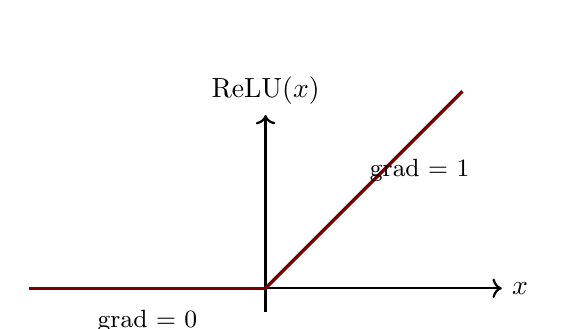
\begin{tikzpicture}
  \draw[->,thick] (-3,0) -- (3,0) node[right] {$x$};
  \draw[->,thick] (0,-0.3) -- (0,2.2) node[above] {ReLU$(x)$};
  \draw[very thick,red] (-3,0) -- (0,0);
  \draw[very thick,red] (0,0) -- (2.5,2.5);
  \node[below,font=\small] at (-1.5,-0.15) {grad = 0};
  \node[right,font=\small] at (1.2,1.5) {grad = 1};
\end{tikzpicture}
\end{center}

\subsection{Derived Operations — No New Math}

\begin{lstlisting}
def __neg__(self):          return self * -1         # negate = multiply by -1
def __radd__(self, other):  return self + other      # fallback for: 2 + a
def __sub__(self, other):   return self + (-other)   # a - b = a + (-b)
def __rsub__(self, other):  return other + (-self)   # fallback for: 2 - a
def __rmul__(self, other):  return self * other      # fallback for: 2 * a
def __truediv__(self, other):   return self * other**-1  # a/b = a * b^(-1)
def __rtruediv__(self, other):  return other * self**-1  # fallback for: 2 / a
def __repr__(self):
    return f"Value(data={self.data}, grad={self.grad})"
\end{lstlisting}

\begin{codeexplainbox}{The \texttt{r*} fallback methods}
Python operator resolution works like this: \code{2 * a} first asks \code{int} to multiply with a \code{Value}, which fails because \code{int} has no idea what a \code{Value} is. Python then falls back to \code{a.\_\_rmul\_\_}. Defining \code{\_\_rmul\_\_} as \code{return self * other} reverses the operands so the call becomes \code{a * 2}, which works.

Without these four \code{r*} methods, expressions like \code{1 - loss} (very common in loss functions), \code{2 * weight}, and \code{0.1 / param} would all crash with \code{TypeError}. They are not optional.
\end{codeexplainbox}

\subsection{Tanh — An Optional Alternative Activation}

\begin{lstlisting}
import math

def tanh(self):
    x = self.data
    t = (math.exp(2*x) - 1) / (math.exp(2*x) + 1)  # compute tanh(x)
    out = Value(t, (self,), 'tanh')

    def _backward():
        # Derivative of tanh: d/dx tanh(x) = 1 - tanh(x)^2
        # t is tanh(x), already computed in forward pass - reuse it here
        self.grad += (1 - t**2) * out.grad

    out._backward = _backward
    return out
\end{lstlisting}

\begin{codeexplainbox}{Abstraction level is a design choice}
You can implement \code{tanh} at two different levels of granularity:

\textbf{Fine-grained:} Implement \code{exp}, then build \code{tanh} from \code{exp}, \code{-}, \code{/}. The computation graph grows: it will have multiple nodes for each intermediate step. But every node is simple, and autograd handles the whole thing.

\textbf{Coarse-grained:} Implement \code{tanh} as one node using its known closed-form derivative $1 - t^2$. The graph has fewer nodes and may run slightly faster. The gradients are identical.

Both approaches give exactly the same gradients at the leaves. Choosing coarse-grained makes sense when you have a reliable formula for the derivative. Choosing fine-grained makes sense when you want maximum flexibility and composability. Neither is wrong.
\end{codeexplainbox}

\begin{mathbox}{tanh derivative}
\[
\frac{d}{dx}\tanh(x) = 1 - \tanh^2(x)
\]
Since $t = \tanh(x)$ is computed during the forward pass and stored as a local variable, the backward reuses it: \code{self.grad += (1 - t**2) * out.grad}. At $x=0$, the derivative is 1 (maximum). At large $|x|$, $\tanh \to \pm 1$ so the derivative $\to 0$ — this is the vanishing gradient problem.
\end{mathbox}

% ═════════════════════════════════════════════════════════════════════════════
\section{The Backward Pass — Topological Order and Chain Rule}
% ═════════════════════════════════════════════════════════════════════════════

\subsection{Why Order Matters}

You cannot call \code{\_backward()} on a node until every node that depends on it has already had its \code{\_backward()} called. Consider $d = c + e$ and $L = d \cdot f$. To compute \code{c.grad}, you need \code{d.grad} to already be filled in. But \code{d.grad} is filled in when \code{L}'s \code{\_backward()} runs. So you must process $L$ before $d$, and $d$ before $c$ and $e$.

This ordering constraint is exactly what \textbf{topological sort} produces: an ordering of all nodes such that every node appears before its inputs.

\subsection{The \texttt{backward()} Method}

\begin{lstlisting}
def backward(self):
    # Phase 1: Build topological ordering of the entire computation graph
    topo = []
    visited = set()

    def build_topo(v):
        if v not in visited:
            visited.add(v)
            for child in v._prev:    # recurse into all inputs (children) first
                build_topo(child)
            topo.append(v)           # only add self AFTER all inputs are done

    build_topo(self)   # start from the output node (e.g. loss)

    # Phase 2: Seed the root gradient
    self.grad = 1   # dL/dL = 1 always - this is the base case

    # Phase 3: Walk backward through the graph, applying each node's backward
    for v in reversed(topo):   # reversed: root first, leaves last
        v._backward()
\end{lstlisting}

\begin{codeexplainbox}{Dissecting build\_topo recursively}
Start at the root (say, \code{loss}). Mark it visited. Recurse into each of its \code{\_prev} children. For each child, mark it visited and recurse into its children. A node is only appended to \code{topo} \emph{after} all its children have been appended.

Result: \code{topo[0]} is a leaf (no parents — it was one of the first to have all children done, which for leaves is trivially true). \code{topo[-1]} is the root.

\code{reversed(topo)} starts at the root and ends at the leaves — exactly the order in which gradients must flow.

The \code{visited} set is essential. Without it, any node used more than once would be added to \code{topo} multiple times and have its \code{\_backward()} called multiple times. The \code{+=} in each \code{\_backward()} would cause gradients to accumulate incorrectly. The \code{visited} set ensures every node's backward runs exactly once.
\end{codeexplainbox}

\begin{stickybox}
\textbf{The complete cycle in one sentence:}
Forward pass builds the graph (by creating \code{Value} nodes and setting their \code{\_backward} closures); \code{loss.backward()} topologically sorts the graph, sets \code{loss.grad=1}, and calls each \code{\_backward()} in reverse order; afterward, every parameter's \code{.grad} holds the correct partial derivative of the loss with respect to that parameter.
\end{stickybox}

% ═════════════════════════════════════════════════════════════════════════════
\section{The Bugs — What Goes Wrong and Why}
% ═════════════════════════════════════════════════════════════════════════════

\subsection{Forgetting to Zero Gradients}

\begin{dangerbox}
\textbf{The most common bug in neural network training.} Every \code{\_backward()} uses \code{+=}. If you call \code{backward()} twice without resetting \code{.grad} to zero between calls, the second backward adds on top of the first. Gradients accumulate indefinitely.

Symptom: the network may seem to converge faster than expected (because the effective step size is inflated by accumulated gradients), then suddenly diverge, or converge to a wrong solution.
\end{dangerbox}

\begin{lstlisting}
# WRONG: gradients from step 0 persist into step 1, 2, 3...
for step in range(100):
    loss = compute_loss(model, xs, ys)
    loss.backward()           # += on already-nonzero grads
    update(model)

# CORRECT: reset before every backward
for step in range(100):
    loss = compute_loss(model, xs, ys)
    for p in model.parameters():
        p.grad = 0            # reset to zero
    loss.backward()           # now accumulates from a clean slate
    update(model)
\end{lstlisting}

\subsection{The Overwrite Bug When a Node Is Used Twice}

\begin{lstlisting}
# Wrong implementation using = instead of +=
def _backward():
    self.grad  = other.data * out.grad   # BUG: overwrites, not accumulates
    other.grad = self.data  * out.grad

# Bug manifests here:
a = Value(3.0)
b = a * a     # a is used as both self AND other
b.backward()
print(a.grad) # should be 2*3 = 6, but wrong impl gives only 3
\end{lstlisting}

When \code{a * a} runs, \code{self} and \code{other} both point to the same object \code{a}. With \code{=}, the second assignment overwrites the first. With \code{+=}, both assignments accumulate, giving the correct result: $2a = 6$. The \code{+=} in \code{\_backward()} is not optional; it is the fix to this fundamental issue.

\subsection{The Sign Bug in the Update}

\begin{lstlisting}
# WRONG: increases the loss
p.data += lr * p.grad   # + sign goes uphill (maximizes L)

# CORRECT: decreases the loss
p.data -= lr * p.grad   # - sign goes downhill (minimizes L)
\end{lstlisting}

The gradient points in the direction that \emph{increases} the loss. Gradient \emph{descent} moves in the opposite direction. The minus sign is the descent. If you get the sign wrong, your network will run gradient \emph{ascent} — the loss will go up, your predictions will get worse, and everything will diverge.

% ═════════════════════════════════════════════════════════════════════════════
\section{The Neural Network Library — nn.py}
% ═════════════════════════════════════════════════════════════════════════════

\subsection{Module — The Base Class}

\begin{lstlisting}
class Module:
    def zero_grad(self):
        for p in self.parameters():
            p.grad = 0      # reset before each backward pass

    def parameters(self):
        return []           # subclasses override to return their trainable params
\end{lstlisting}

\begin{codeexplainbox}{Why have a base class at all}
\code{Module} exists so that every object in the hierarchy — \code{Neuron}, \code{Layer}, \code{MLP} — has the same interface. You can call \code{model.zero\_grad()} and \code{model.parameters()} on any of them, regardless of internal complexity.

This mirrors \code{torch.nn.Module} in PyTorch exactly. The design choice is deliberate: learning micrograd gives you the mental model for PyTorch's module system.

The default \code{parameters()} returns \code{[]}, encoding the assumption that a bare \code{Module} has nothing trainable. Subclasses override this to return their actual \code{Value} objects.
\end{codeexplainbox}

\subsection{Neuron — The Atom}

\begin{lstlisting}
class Neuron(Module):

    def __init__(self, nin, nonlin=True):
        # nin: number of inputs to this neuron
        self.w = [Value(random.uniform(-1, 1)) for _ in range(nin)]
        self.b = Value(0)        # bias: starts at zero
        self.nonlin = nonlin     # whether to apply ReLU after the linear combination

    def __call__(self, x):
        # Compute: w*x + b  (dot product of weights and inputs, plus bias)
        # sum(..., start) starts the accumulation from self.b (a Value)
        # This ensures the entire sum is a Value object, not a plain float
        act = sum((wi * xi for wi, xi in zip(self.w, x)), self.b)
        return act.relu() if self.nonlin else act

    def parameters(self):
        return self.w + [self.b]   # nin weights + 1 bias = nin+1 params total

    def __repr__(self):
        return f"{'ReLU' if self.nonlin else 'Linear'}Neuron({len(self.w)})"
\end{lstlisting}

\begin{codeexplainbox}{Every decision in Neuron}

\textbf{Random initialization:} Weights are sampled from $\text{Uniform}(-1, 1)$. If all weights started at zero, every neuron in a layer would compute the same output and receive the same gradient — they would forever remain identical. Random initialization breaks this symmetry.

\textbf{Bias starts at zero:} The bias shifts the activation function left or right. Zero is a neutral starting point — the network learns the right offset during training.

\textbf{\code{sum(..., self.b)} — the start parameter:} Python's built-in \code{sum(iterable, start=0)} starts accumulating from \code{start}. If you leave the default \code{start=0} (a plain Python int), the first addition would be \code{int + Value}, which triggers \code{int.\_\_add\_\_(Value)}, which fails. By passing \code{self.b} (a \code{Value}) as the start, all arithmetic stays within the \code{Value} universe. Every intermediate result remains a \code{Value}, and every operation is tracked in the graph.

\textbf{\code{zip(self.w, x)}:} Pairs each weight with the corresponding input: \code{[(w0,x0), (w1,x1), ...]}. The generator expression \code{(wi * xi for wi, xi in zip(self.w, x))} produces the products lazily, and \code{sum} accumulates them.

\textbf{\code{nonlin=False} for the output layer:} The output should be raw numbers (logits) so the loss function receives unrestricted values. Applying ReLU to the output would clamp negatives to zero, breaking the gradient signal. Always pass \code{nonlin=False} to the last layer.

\textbf{What \code{\_\_call\_\_} does:} When you write \code{neuron(x)}, Python internally calls \code{neuron.\_\_call\_\_(x)}. This means neurons are callable objects — they look and behave like functions while being full objects with learnable state.
\end{codeexplainbox}

\begin{mathbox}{The neuron's computation}
\[
\text{output} = \text{ReLU}\!\left(\sum_{i=1}^{n} w_i x_i + b\right)
\]
The sum $\sum w_i x_i + b$ is the linear combination. The ReLU is the nonlinearity. Without the nonlinearity, stacking multiple layers would be equivalent to a single layer (a composition of linear functions is linear). The nonlinearity is what makes deep networks expressively more powerful than shallow ones.
\end{mathbox}

\subsection{Layer — A Row of Independent Neurons}

\begin{lstlisting}
class Layer(Module):

    def __init__(self, nin, nout, **kwargs):
        # nin: input dimension for each neuron
        # nout: how many neurons in this layer
        # **kwargs: passed straight through to Neuron (e.g. nonlin=False)
        self.neurons = [Neuron(nin, **kwargs) for _ in range(nout)]

    def __call__(self, x):
        # All neurons see the same input x, compute independently
        out = [n(x) for n in self.neurons]
        # Convenience: if there is only one output, unwrap from list
        return out[0] if len(out) == 1 else out

    def parameters(self):
        # Flatten: for each neuron, collect its parameters; combine all
        return [p for n in self.neurons for p in n.parameters()]

    def __repr__(self):
        return f"Layer of [{', '.join(str(n) for n in self.neurons)}]"
\end{lstlisting}

\begin{codeexplainbox}{Layer design decisions}

\textbf{All neurons see the same input:} This is the definition of a fully-connected (dense) layer. Input $x$ is broadcast to every neuron. Each neuron has its own independent weights and bias — they are not shared.

\textbf{Outputs are computed independently:} In a real library, this would happen in parallel (vectorized over a matrix). In micrograd, it is a list comprehension — conceptually equivalent but sequential.

\textbf{\code{**kwargs} pass-through:} The keyword argument \code{nonlin=False} needs to reach the individual neurons of the last layer. By using \code{**kwargs}, \code{Layer} can accept arbitrary extra arguments and forward them to each \code{Neuron} constructor without knowing what those arguments mean.

\textbf{Flattened \code{parameters()}:} The nested list comprehension \code{[p for n in self.neurons for p in n.parameters()]} reads as: for each neuron, get its parameter list; pool all parameter lists into a single flat list. This lets \code{model.parameters()} at the top level return everything as one flat iterable.

\textbf{Single-output unwrap:} The output layer typically has exactly one neuron (for binary classification or regression). In that case, returning a list of one element would be awkward. The \code{return out[0] if len(out) == 1 else out} handles this gracefully.
\end{codeexplainbox}

\subsection{MLP — The Full Architecture}

\begin{lstlisting}
class MLP(Module):

    def __init__(self, nin, nouts):
        # nin: number of input features (e.g., 3 for a 3D input)
        # nouts: list of layer sizes [hidden1, hidden2, ..., output]
        # Example: MLP(3, [4, 4, 1]) means 3 inputs -> 4 -> 4 -> 1 output

        sz = [nin] + nouts   # e.g., [3, 4, 4, 1]

        # Create layers from consecutive pairs of sizes
        # Layer(3,4): first layer  Layer(4,4): second  Layer(4,1): output
        self.layers = [
            Layer(sz[i], sz[i+1], nonlin=(i != len(nouts)-1))
            for i in range(len(nouts))
        ]
        # nonlin=True for all layers except the last one (i != len(nouts)-1)

    def __call__(self, x):
        # Feed-forward: output of each layer becomes input of the next
        for layer in self.layers:
            x = layer(x)
        return x

    def parameters(self):
        return [p for layer in self.layers for p in layer.parameters()]

    def __repr__(self):
        return f"MLP of [{', '.join(str(layer) for layer in self.layers)}]"
\end{lstlisting}

\begin{codeexplainbox}{The sz trick and the nonlin condition}

\textbf{\code{sz = [nin] + nouts}:} This prepends the input dimension to the list of layer sizes. For \code{MLP(3, [4, 4, 1])}: \code{sz = [3, 4, 4, 1]}. Then \code{sz[i]} and \code{sz[i+1]} form consecutive pairs: \code{(3,4)}, \code{(4,4)}, \code{(4,1)} — exactly the input and output size of each successive layer.

\textbf{\code{nonlin=(i != len(nouts)-1)}:} This boolean expression is \code{True} for every layer except the last one. \code{len(nouts)-1} is the index of the last layer. At that index, \code{i == len(nouts)-1}, so the expression is \code{False}, disabling the nonlinearity. Every hidden layer gets ReLU; the output layer does not.

\textbf{Sequential \code{\_\_call\_\_}:} The loop \code{for layer in self.layers: x = layer(x)} is the entire forward pass. The output of layer $i$ replaces \code{x} and becomes the input to layer $i+1$. After the loop, \code{x} is the final output.

\textbf{Flat \code{parameters()}:} The same nested list comprehension pattern as in \code{Layer}, but one level deeper. For \code{MLP(3, [4, 4, 1])}: 3 layers, each with several neurons, each with several parameters. All of them end up in one flat list — 41 total for this configuration.
\end{codeexplainbox}

\begin{center}
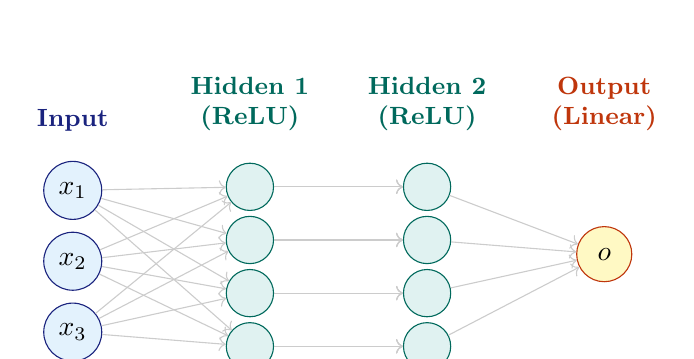
\begin{tikzpicture}[node distance=0.45cm and 1.5cm, scale=0.9]
  \foreach \i in {1,2,3} {
    \node[circle,draw=deepblue,fill=noteblue,minimum size=0.6cm] (x\i) at (0,-\i) {$x_\i$};
  }
  \foreach \i in {1,2,3,4} {
    \node[circle,draw=teal,fill=conceptbg,minimum size=0.6cm] (h1\i) at (2.5,-\i*0.75-0.2) {};
  }
  \foreach \i in {1,2,3,4} {
    \node[circle,draw=teal,fill=conceptbg,minimum size=0.6cm] (h2\i) at (5,-\i*0.75-0.2) {};
  }
  \node[circle,draw=orange,fill=warnbg,minimum size=0.7cm] (out) at (7.5,-1.9) {$o$};
  \foreach \i in {1,2,3} \foreach \j in {1,2,3,4} {
    \draw[->,gray!40] (x\i) -- (h1\j);
    \draw[->,gray!40] (h1\j) -- (h2\j);
  }
  \foreach \j in {1,2,3,4} \draw[->,gray!40] (h2\j) -- (out);
  \node[above,font=\small\bfseries\color{deepblue}] at (0,-0.3) {Input};
  \node[above,font=\small\bfseries\color{teal},align=center] at (2.5,-0.3) {Hidden 1\\(ReLU)};
  \node[above,font=\small\bfseries\color{teal},align=center] at (5,-0.3) {Hidden 2\\(ReLU)};
  \node[above,font=\small\bfseries\color{orange},align=center] at (7.5,-0.3) {Output\\(Linear)};
\end{tikzpicture}
\end{center}

% ═════════════════════════════════════════════════════════════════════════════
\section{The Training Loop — Everything Together}
% ═════════════════════════════════════════════════════════════════════════════

\subsection{The Dataset and Loss}

\begin{lstlisting}
# 4 training examples, 3 features each
xs = [
    [2.0,  3.0, -1.0],
    [3.0, -1.0,  0.5],
    [0.5,  1.0,  1.0],
    [1.0,  1.0, -1.0],
]
ys = [1.0, -1.0, -1.0, 1.0]   # binary targets: +1 or -1

model = MLP(3, [4, 4, 1])
print(f"Parameters: {len(model.parameters())}")  # 41
\end{lstlisting}

\begin{lstlisting}
# Forward pass: get predictions for all examples
ypred = [model(x) for x in xs]

# Mean Squared Error loss: each term is a Value object
# Because ypred contains Value objects, every arithmetic op here is tracked
loss = sum((yout - ygt)**2 for ygt, yout in zip(ys, ypred))

# loss is now a single Value at the tip of a massive computation graph
# Calling loss.backward() will propagate gradients through the entire graph
print(loss.data)   # e.g., 7.12
\end{lstlisting}

\begin{mathbox}{Mean Squared Error}
\[
L = \sum_{i=1}^{N} (\hat{y}_i - y_i)^2
\]
\begin{itemize}
  \item $\hat{y}_i$: model prediction for example $i$ (a \code{Value} object)
  \item $y_i$: ground truth target (a plain Python float)
  \item When \code{yout - ygt} runs: \code{ygt} is a float, so Python tries \code{float.\_\_sub\_\_(Value)}, fails, then falls back to \code{Value.\_\_rsub\_\_(float)}, which succeeds
  \item The result is a \code{Value}; squaring it via \code{**2} creates another \code{Value}; summing all creates the final \code{loss} \code{Value}
\end{itemize}
The loss is zero only when every prediction exactly matches its target. Any mismatch produces a positive contribution. Minimizing $L$ pushes all predictions toward their targets simultaneously.
\end{mathbox}

\subsection{The Training Loop}

\begin{lstlisting}
model = MLP(3, [4, 4, 1])
learning_rate = 0.05

for step in range(50):

    # -- 1. FORWARD PASS --------------------------------------------------
    # Run all examples through the model
    # Each model(x) call builds a computation subgraph
    # All subgraphs share the same weight nodes
    ypred = [model(x) for x in xs]
    loss  = sum((yout - ygt)**2 for ygt, yout in zip(ys, ypred))

    # -- 2. ZERO GRADIENTS ------------------------------------------------
    # MUST come before backward, not after
    # All _backward() use +=, so old gradients would corrupt new ones
    for p in model.parameters():
        p.grad = 0

    # -- 3. BACKWARD PASS -------------------------------------------------
    # Topological sort + chain rule
    # After this, every p in model.parameters() has a correct p.grad
    loss.backward()

    # -- 4. GRADIENT DESCENT UPDATE ---------------------------------------
    # Subtract: go against the gradient to minimize the loss
    # The - sign is not optional: + would maximize the loss
    for p in model.parameters():
        p.data -= learning_rate * p.grad

    if step % 10 == 0:
        preds_str = [f"{y.data:.3f}" for y in ypred]
        print(f"step {step:3d} | loss = {loss.data:.6f} | preds = {preds_str}")
\end{lstlisting}

\begin{codeexplainbox}{Reading the training loop as a rhythm}
There are exactly four steps, in exactly this order, on every iteration:

\textbf{Forward:} Run inputs through the model. A new computation graph is built each time. The weights (\code{p.data}) are the shared nodes that persist across iterations. The intermediate nodes (activations) are freshly created each step.

\textbf{Zero grad:} Reset all \code{.grad} fields to zero. This must happen before \code{backward()}, not after. If you do it after, the gradients sit at zero throughout the entire update step, which is actually fine — but then you lose the gradient information before you've used it. Standard practice: zero first, then backward, then update.

\textbf{Backward:} \code{loss.backward()} runs the topological sort on the current graph and calls every \code{\_backward()} closure in reverse order. After this call returns, every parameter's \code{.grad} holds exactly $\frac{\partial L}{\partial p}$ for this batch of examples and this configuration of weights.

\textbf{Update:} \code{p.data -= lr * p.grad}. The learning rate \code{lr} controls the step size. Too large: you overshoot and the loss explodes. Too small: convergence is very slow. The minus sign makes the update go downhill.
\end{codeexplainbox}

\begin{mathbox}{Gradient Descent}
\[
p \leftarrow p - \eta \cdot \frac{\partial L}{\partial p}
\]
$\eta$ (eta) is the learning rate. The gradient $\frac{\partial L}{\partial p}$ points in the direction of steepest \emph{increase} of the loss. Subtracting it moves $p$ in the direction of steepest decrease — downhill on the loss surface.
\end{mathbox}

\begin{warnbox}
\textbf{Learning rate sensitivity.} If \code{lr = 0.5} causes the loss to oscillate or grow, try \code{lr = 0.05} or \code{lr = 0.01}. A typical sign of too-large LR is the loss bouncing up and down each step. A typical sign of too-small LR is the loss barely decreasing after many steps.
\end{warnbox}

% ═════════════════════════════════════════════════════════════════════════════
\section{Connecting to PyTorch}
% ═════════════════════════════════════════════════════════════════════════════

\begin{lstlisting}
import torch

# Scalar values as 1-element tensors; .double() for float64 (like Python floats)
x1 = torch.Tensor([2.0]).double();  x1.requires_grad = True
x2 = torch.Tensor([0.0]).double();  x2.requires_grad = True
w1 = torch.Tensor([-3.0]).double(); w1.requires_grad = True
w2 = torch.Tensor([1.0]).double();  w2.requires_grad = True
b  = torch.Tensor([6.8813735870195432]).double(); b.requires_grad = True

n  = x1*w1 + x2*w2 + b
o  = torch.tanh(n)           # PyTorch has tanh built in

o.backward()                  # same call as micrograd

# .item() extracts the scalar from a single-element tensor
print(o.data.item())          # 0.7071 - same as micrograd
print(x2.grad.item())         # 0.5
print(w2.grad.item())         # 0.0
print(x1.grad.item())         # -1.5
print(w1.grad.item())         # 1.0
# All identical to micrograd results
\end{lstlisting}

\begin{tipbox}
\textbf{The differences between micrograd and PyTorch:}

\textbf{Tensors vs scalars:} PyTorch wraps $n$-dimensional arrays; micrograd wraps single numbers. The math is the same. \code{.item()} extracts one number from a tensor.

\textbf{\code{requires\_grad=False} by default:} PyTorch optimizes by not tracking gradients unless you ask. Leaf nodes that are inputs (data, not parameters) usually don't need gradients. Only parameters get \code{requires\_grad=True}.

\textbf{\code{float32} vs \code{float64}:} PyTorch defaults to 32-bit floats for speed on GPUs. Python uses 64-bit floats. Cast with \code{.double()} to match.

\textbf{API compatibility:} \code{.backward()}, \code{.grad}, \code{.data}, \code{torch.nn.Module}, \code{.zero\_grad()}, \code{.parameters()} — all these exist in both micrograd and PyTorch, with identical semantics. Learning micrograd means you already know the PyTorch API conceptually.
\end{tipbox}

% ═════════════════════════════════════════════════════════════════════════════
\section{The Complete Annotated Source}
% ═════════════════════════════════════════════════════════════════════════════

\subsection{engine.py}

\begin{lstlisting}
class Value:
    """
    A node in the computation graph.
    Wraps one scalar, tracks how it was produced, and stores its gradient.
    """

    def __init__(self, data, _children=(), _op=''):
        self.data = data                      # the scalar value
        self.grad = 0                         # dL/dself; filled by backward()
        self._backward = lambda: None         # closure set by each op; default no-op
        self._prev = set(_children)           # set of input nodes that produced self
        self._op = _op                        # string label for debugging

    # -- FORWARD OPERATIONS + BACKWARD REGISTRATION -----------------------

    def __add__(self, other):
        other = other if isinstance(other, Value) else Value(other)
        out = Value(self.data + other.data, (self, other), '+')

        def _backward():
            # d(self + other)/d(self) = 1   ->  self.grad += 1 * out.grad
            # d(self + other)/d(other) = 1  ->  other.grad += 1 * out.grad
            self.grad  += out.grad
            other.grad += out.grad

        out._backward = _backward
        return out

    def __mul__(self, other):
        other = other if isinstance(other, Value) else Value(other)
        out = Value(self.data * other.data, (self, other), '*')

        def _backward():
            # d(self * other)/d(self) = other  -> self.grad += other.data * out.grad
            # d(self * other)/d(other) = self  -> other.grad += self.data * out.grad
            self.grad  += other.data * out.grad
            other.grad += self.data  * out.grad

        out._backward = _backward
        return out

    def __pow__(self, other):
        assert isinstance(other, (int, float))   # exponent must be a constant
        out = Value(self.data**other, (self,), f'**{other}')

        def _backward():
            # Power rule: d/dx [x^n] = n * x^(n-1)
            self.grad += (other * self.data**(other - 1)) * out.grad

        out._backward = _backward
        return out

    def relu(self):
        out = Value(0 if self.data < 0 else self.data, (self,), 'ReLU')

        def _backward():
            # Derivative: 1 if output > 0, else 0
            # (out.data > 0) is True (=1) or False (=0)
            self.grad += (out.data > 0) * out.grad

        out._backward = _backward
        return out

    # -- TOPOLOGICAL SORT + CHAIN RULE APPLICATION ------------------------

    def backward(self):
        topo, visited = [], set()

        def build_topo(v):
            if v not in visited:
                visited.add(v)
                for child in v._prev:
                    build_topo(child)
                topo.append(v)   # self added only after all inputs are done

        build_topo(self)

        self.grad = 1            # base case: dL/dL = 1
        for v in reversed(topo):
            v._backward()        # each node deposits gradient into its inputs

    # -- DERIVED OPERATIONS - reuse existing backward logic ----------------

    def __neg__(self):          return self * -1
    def __radd__(self, other):  return self + other      # handles: 2 + a
    def __sub__(self, other):   return self + (-other)
    def __rsub__(self, other):  return other + (-self)   # handles: 2 - a
    def __rmul__(self, other):  return self * other      # handles: 2 * a
    def __truediv__(self, other):   return self * other**-1
    def __rtruediv__(self, other):  return other * self**-1  # handles: 2 / a

    def __repr__(self):
        return f"Value(data={self.data}, grad={self.grad})"
\end{lstlisting}

\subsection{nn.py}

\begin{lstlisting}
import random
from micrograd.engine import Value


class Module:
    """Base class for all neural network components."""

    def zero_grad(self):
        for p in self.parameters():
            p.grad = 0    # reset gradient before each backward pass

    def parameters(self):
        return []         # subclasses override to return their Value objects


class Neuron(Module):
    """
    Single artificial neuron.
    Computes: ReLU(w*x + b)  or  w*x + b  (if nonlin=False)
    """

    def __init__(self, nin, nonlin=True):
        # nin weights, one per input dimension
        self.w = [Value(random.uniform(-1, 1)) for _ in range(nin)]
        self.b = Value(0)        # bias initialized to zero
        self.nonlin = nonlin     # controls whether ReLU is applied

    def __call__(self, x):
        # sum(..., start=self.b): accumulates wi*xi values into a Value
        # Starting from self.b (a Value) ensures the result stays a Value
        act = sum((wi * xi for wi, xi in zip(self.w, x)), self.b)
        return act.relu() if self.nonlin else act

    def parameters(self):
        return self.w + [self.b]   # nin+1 trainable scalars

    def __repr__(self):
        return f"{'ReLU' if self.nonlin else 'Linear'}Neuron({len(self.w)})"


class Layer(Module):
    """
    A fully-connected layer: nout independent neurons, each seeing the same input.
    """

    def __init__(self, nin, nout, **kwargs):
        self.neurons = [Neuron(nin, **kwargs) for _ in range(nout)]

    def __call__(self, x):
        out = [n(x) for n in self.neurons]
        return out[0] if len(out) == 1 else out  # unwrap single-neuron layers

    def parameters(self):
        # Flatten: all parameters from all neurons into one list
        return [p for n in self.neurons for p in n.parameters()]

    def __repr__(self):
        return f"Layer of [{', '.join(str(n) for n in self.neurons)}]"


class MLP(Module):
    """
    Multi-Layer Perceptron: a sequence of fully-connected layers.
    Each layer's output feeds the next layer's input.
    """

    def __init__(self, nin, nouts):
        sz = [nin] + nouts  # e.g., MLP(3, [4,4,1]) -> sz = [3, 4, 4, 1]
        self.layers = [
            Layer(sz[i], sz[i+1], nonlin=(i != len(nouts)-1))
            for i in range(len(nouts))
        ]
        # nonlin is True for hidden layers, False only for the last layer

    def __call__(self, x):
        for layer in self.layers:
            x = layer(x)   # feed-forward: output of layer i -> input of layer i+1
        return x

    def parameters(self):
        return [p for layer in self.layers for p in layer.parameters()]

    def __repr__(self):
        return f"MLP of [{', '.join(str(layer) for layer in self.layers)}]"
\end{lstlisting}

% ═════════════════════════════════════════════════════════════════════════════
\section{Complete Reference — Sticky Points}
% ═════════════════════════════════════════════════════════════════════════════

\begin{stickybox}
\textbf{1. What a \texttt{Value} holds.}\\
\code{.data}: the number. \code{.grad}: $\partial L / \partial$self. \code{.\_backward}: closure for gradient propagation. \code{.\_prev}: input nodes. \code{.\_op}: label.
\end{stickybox}

\begin{stickybox}
\textbf{2. \texttt{.grad} starts at 0.}\\
Encodes ``no effect assumed.'' Backward accumulates via \code{+=} to fill in the real value. If a node is unreachable, grad stays 0 — correctly.
\end{stickybox}

\begin{stickybox}
\textbf{3. Always \texttt{+=} in backward.}\\
Multiple uses of the same node each contribute a gradient. \code{+=} accumulates all contributions. \code{=} would overwrite them — wrong.
\end{stickybox}

\begin{stickybox}
\textbf{4. Closures capture references.}\\
\code{\_backward} captures \code{self}, \code{other}, \code{out} by reference, not by copy. When called later, it reads their current state (including updated \code{.grad} fields).
\end{stickybox}

\begin{stickybox}
\textbf{5. Zero grad before backward.}\\
\code{p.grad = 0} for all parameters before every \code{loss.backward()}. Without this, gradients accumulate across training steps.
\end{stickybox}

\begin{stickybox}
\textbf{6. Topological order is mandatory.}\\
Process a node's backward only after all nodes that \emph{depend on it} have been processed. \code{build\_topo} guarantees this.
\end{stickybox}

\begin{stickybox}
\textbf{7. $+$ distributes gradient.}\\
$c = a + b$: both $a$ and $b$ receive \code{c.grad} unchanged. A plus node fans out the upstream gradient to all its inputs equally.
\end{stickybox}

\begin{stickybox}
\textbf{8. $\times$ swaps and scales.}\\
$c = a \times b$: \code{a.grad += b.data * c.grad}, \code{b.grad += a.data * c.grad}. Each input's gradient is scaled by the other's forward value.
\end{stickybox}

\begin{stickybox}
\textbf{9. Division is power rule.}\\
\code{a / b} → \code{a * b**-1} → power rule on \code{b}. No new backward logic.
\end{stickybox}

\begin{stickybox}
\textbf{10. ReLU gates gradient.}\\
\code{(out.data > 0) * out.grad}: gradient flows if forward output was positive, blocked if zero or negative.
\end{stickybox}

\begin{stickybox}
\textbf{11. Seed \texttt{loss.grad = 1}.}\\
$\partial L / \partial L = 1$ always. This is the base case. Everything else is derived from it via the chain rule.
\end{stickybox}

\begin{stickybox}
\textbf{12. Minus sign in update.}\\
\code{p.data -= lr * p.grad}. Gradient points uphill; subtract to go downhill and minimize the loss.
\end{stickybox}

\begin{stickybox}
\textbf{13. r* methods are essential.}\\
Without \code{\_\_radd\_\_}, \code{\_\_rmul\_\_}, etc., expressions like \code{1 - loss} and \code{2 * weight} crash. They reverse operand order when Python's normal dispatch fails.
\end{stickybox}

\begin{stickybox}
\textbf{14. \texttt{sum(..., self.b)} trick.}\\
Starts accumulation from a \code{Value} (the bias), keeping all arithmetic in the \code{Value} graph. Starting from \code{0} (int) would break the first \code{Value +} call.
\end{stickybox}

\begin{stickybox}
\textbf{15. \texttt{nonlin=False} for last layer.}\\
Output neurons produce raw values. ReLU on the output would clamp negatives to zero and destroy gradient signal into the loss.
\end{stickybox}

\begin{stickybox}
\textbf{16. \texttt{sz = [nin] + nouts}.}\\
Prepend input dim to get full size list. Consecutive pairs \code{(sz[i], sz[i+1])} define each layer's shape.
\end{stickybox}

\begin{stickybox}
\textbf{17. Abstraction level is flexible.}\\
Any differentiable function can be a node. Fine-grained (many small ops) and coarse-grained (one op with a known derivative) give identical gradients.
\end{stickybox}

\begin{stickybox}
\textbf{18. PyTorch is micrograd + efficiency.}\\
Tensors = batches of scalars. GPU kernels = fast matmul. \code{requires\_grad} = selective tracking. The math is identical.
\end{stickybox}

% ═════════════════════════════════════════════════════════════════════════════
\section{Reading Code as a Mental Simulation}
% ═════════════════════════════════════════════════════════════════════════════

Developing strong code-writing intuition means being able to mentally simulate execution. For autograd code specifically, practice the following on any expression you write:

\subsection{The Forward-Pass Trace}

Given any expression, identify: which \code{Value} objects exist, what their \code{.data} values are, what their \code{.\_prev} sets contain, and what closure is stored in each \code{.\_backward}.

Example: trace \code{c = a + b} where \code{a = Value(2.0)} and \code{b = Value(-3.0)}.
\begin{itemize}
  \item \code{c.data = -1.0}
  \item \code{c.\_prev = \{a, b\}}
  \item \code{c.\_op = '+'}
  \item \code{c.\_backward} is a closure capturing \code{self=a}, \code{other=b}, \code{out=c}
  \item When called: \code{a.grad += c.grad}, \code{b.grad += c.grad}
\end{itemize}

\subsection{The Backward-Pass Trace}

Starting from \code{c.grad = 1}, call \code{c.\_backward()}. Deposit \code{1} into both \code{a.grad} and \code{b.grad}. Both are leaves (no \code{\_prev}), so their \code{\_backward} is the no-op lambda. Backward terminates.

For a deeper expression, always work backwards from the output node, calling each closure in topological-reverse order. Draw the graph if needed and annotate \code{.grad} at each step.

\subsection{Identifying Bugs by Pattern}

\begin{itemize}
  \item \textbf{Loss explodes or oscillates:} learning rate too high, or zero-grad missing
  \item \textbf{Loss decreases too slowly or stalls:} learning rate too low, or sign of update reversed
  \item \textbf{Gradients are double what expected:} zero-grad not called, old gradients accumulating
  \item \textbf{Node used twice gives wrong gradient:} \code{=} instead of \code{+=} in \code{\_backward}
  \item \textbf{TypeError on \texttt{2 * a}:} missing \code{\_\_rmul\_\_}
  \item \textbf{sum() returns float not Value:} start parameter of \code{sum} is an int, not \code{self.b}
\end{itemize}

\subsection{Writing New Operations}

Follow the template exactly:

\begin{lstlisting}
def your_op(self, other_args):
    # 1. Compute forward value
    result_data = ...

    # 2. Create output node
    out = Value(result_data, (self,), 'your_op_name')

    # 3. Define backward closure
    def _backward():
        # local derivative of your_op w.r.t. self
        local_grad = ...
        self.grad += local_grad * out.grad   # always +=, never =

    # 4. Attach and return
    out._backward = _backward
    return out
\end{lstlisting}

The only part that changes between operations is \code{local\_grad}. That is the derivative of your operation with respect to its input, evaluated at the forward value. Everything else is boilerplate.

% ═════════════════════════════════════════════════════════════════════════════
\section{Mental Model — The Three Questions}
% ═════════════════════════════════════════════════════════════════════════════

\begin{conceptbox}{At any node in the graph, backpropagation answers three questions}
\begin{enumerate}
  \item \textbf{What did I output?} — stored in \code{.data}, computed during the forward pass
  \item \textbf{How much does the final loss change when my output changes?} — stored in \code{.grad}, deposited by the node downstream of me
  \item \textbf{How much does my output change when each of my inputs changes?} — the local derivative, computed analytically based on my operation type
\end{enumerate}
Multiply answers 2 and 3 → deposit into each input's \code{.grad} using \code{+=}. Done.
\end{conceptbox}

\begin{center}
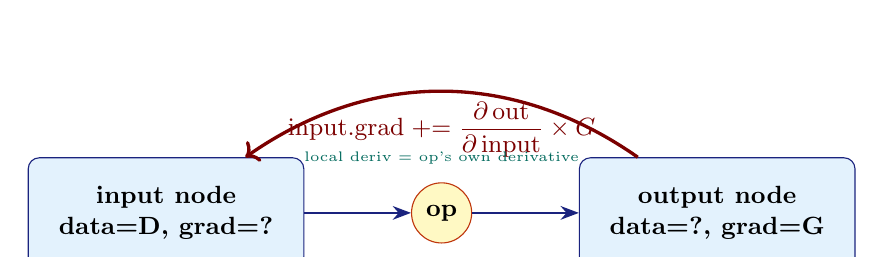
\begin{tikzpicture}
  \node[valnode,minimum width=3.5cm] (inp) at (0,0) {input node\\data=D, grad=?};
  \node[opnode] (op) at (3.5,0) {op};
  \node[valnode,minimum width=3.5cm] (out) at (7,0) {output node\\data=?, grad=G};
  \draw[arr] (inp) -- (op);
  \draw[arr] (op) -- (out);
  \draw[->,very thick,red,bend right=35] (out) to
    node[below,font=\small\color{red},align=center]
    {$\text{input.grad} \mathrel{+}= \dfrac{\partial\,\text{out}}{\partial\,\text{input}} \times G$}
    (inp);
  \node[above,font=\tiny\color{teal}] at (3.5,0.5) {local deriv = op's own derivative};
\end{tikzpicture}
\end{center}

\begin{conceptbox}{Why 100 lines is enough}
The forward pass is just Python arithmetic on \code{Value} objects — the graph builds itself.

The backward pass is one call: \code{loss.backward()} sorts the graph and runs all the closures.

The update is one loop: subtract \code{lr * grad} from each parameter.

Everything else in a production library — tensor operations, GPU kernels, memory management, batching, distributed training — is efficiency. The underlying mathematics is exactly what these 100 lines encode.
\end{conceptbox}

\vfill
\begin{center}
{\small\color{gray}\itshape
Notes by Vatsav Reddy $\cdot$ Under Prof.\ Praveen Parchuri $\cdot$
Reference: A.\ Karpathy's ``Building Micrograd'' lecture $\cdot$
Micrograd source: \texttt{github.com/karpathy/micrograd}
}
\end{center}

\end{document}
